% -- NAO MUDAR O TAMANHO DA FONTE.
% -- O USO DO TAMANHO DA FONTE EM 12PT Eh OBRIGATORIO
\documentclass[12pt]{article}

% -- O USO DO TEMPLATE DA SBC Eh OBRIGATORIO
% -- NAO ALTERAR NENHUMA PARAMETRO DO MODELO DA SBC
% -- (E.G., MARGENS LATERAIS, RODAPE, CABECA�HO, ENTRE OUTROS)
\usepackage{sbc-template}

\usepackage{graphicx,url}
\usepackage{float}

%\usepackage[brazil]{babel}
\usepackage[latin1]{inputenc}

% descomente abaixo caso tenha problemas com a numera��o das se��es n�o
% aparecerem. Em especial no Ububtu 16.x
%\usepackage{etoolbox}
%\makeatletter
%\patchcmd{\ttlh@hang}{\parindent\z@}{\parindent\z@\leavevmode}{}{}
%\patchcmd{\ttlh@hang}{\noindent}{}{}{}
%\makeatother

% -- O USO DESTE COMANDO Eh OBRIGATORIO
\sloppy

% -- CERTIFIQUE-SE DE QUE O TITULO NAO ESTEJA ULTRAPASSANDO OS LIMITES
% -- DAS MARGENS.
% -- USE O COMANDO QUEBRA-DE-LINHA (\\) SE TITULO FOR MUITO LONGO.
\title{Efficient Visual Attention with Deep Learning}

% -- CERTIFIQUE-SE DE QUE O NOME DOS AUTORES ESTEJA CORRETO.
% -- EM GERAL COLOCA-SE O ALUNO COMO PRIMEIRO AUTOR E O ORIENTADOR COMO
% -- ULTIMO AUTOR.
\author{Erik Perillo\inst{1}, Esther Luna Colombini\inst{1}}

% -- CERTIFIQUE-SE DE QUE OS NOMES DAS INSTITUICOES E SEUS RESPECTIVOS ENDERECOS
% -- NAO ESTEJAM ULTRAPASSANDO OS LIMITES DAS MARGENS. SE ISTO OCORRER, USE O
% -- COMANDO QUEBRA-DE-LINHA (\\) OU ABREVIACOES APROPRIADAS.
\address{Institute of Computing (IC) -- University of Campinas
  (Unicamp)\\
  Caixa Postal 6176 -- 13.084-971 -- Campinas -- SP -- Brazil
  \email{erik.perillo@gmail.com, esther@ic.unicamp.br}
}


% -- CERTIFIQUE-SE DE QUE AS TABELAS E FIGURAS INSERIDAS NO
% -- DOCUMENTO NAO ESTEJAM ULTRAPASSANDO
% -- OS LIMITES DAS MARGENS.

\begin{document}

\maketitle

% -- O RESUMO EM INGLES Eh OBRIGATORIO,
% -- INDEPENDENTE DO IDIOMA EM QUE TRABALHO FOI ESCRITO
\begin{abstract}
The high volume of visual data usually available for autonomous applications contains information that is
mostly irrelevant for intelligent agents. Humans perform sensorial filtering through a mechanism called attention. In this work, we present a new fully convolutional neural network architecture designed for detecting visual salience. Experiments carried out with the MIT300 benchmark presented state-of-the-art performance and a parameter reduction of 3/4 compared to similar models.
\end{abstract}

% -- O RESUMO EM PORTUGUES Eh OBRIGATORIO, INDEPENDENTE DO
% -- INDIOMA EM QUE O TRABALHO FOI ESCRITO
\begin{resumo}
O alto volume de dados visuais geralmente dispon�vel para aplica��es aut�nomas cont�m informa��es que s�o, em sua grande parte,  irrelevantes para agentes inteligentes. Os seres humanos realizam uma filtragem sensorial atrav�s de um mecanismo chamado aten��o. Este trabalho descreve uma nova arquitetura de rede neural convolucional projetada para detectar a sali�ncia visual. Os experimentos realizados com o benchmark MIT300 apresentaram desempenho compat�vel com os melhores modelos e uma redu��o de par�metros de 3/4 em compara��o com modelos similares.
\end{resumo}

\section{Introduction}
%\vspace{-0.3cm}
One of the most challenging unsolved problems in Artificial Intelligence is vision.
However, it is fundamental for the conception of systems that interact with the real
physical world. These systems would be useful for applications such as service
robots operating in houses, industry and agriculture, with great potential for the benefit of society.

Vision is remarkably data and computationally intensive.
In humans, approximately half of the brain is involved in
vision-related tasks~\cite{fixott_1957}.
Even our minds can not handle all the sheer amount of sensorial information
received every second. In order to deal with this immense amount of data, we have attentional systems, a fundamental mechanism
that, among other functions, filters out irrelevant information
-- either visual or from other senses-- and helps us focusing our cognitive
processes on what is important at a given moment.
These facts are a strong evidence that, in order to help solving the
vision problems, attention should be applied.

Visual attention can be defined as the delimitation of a certain spatial
region on an image for further cognitive processing~\cite{treisman_1980}.
The phenomenon emerges from two fundamentally different processes:
the \emph{top-down} mechanism that implements our longer-term cognitive strategies by biasing attention according to our interests (e.g. find a red apple in a tree because of hunger,
which will make red be more recognizable on the scene),
and the \emph{bottom-up} mechanism~\cite{colombini_2016}, a process generated through external stimuli
that captures one's attention from its conspicuousness level.
In this work, we focus on the latter, also named visual saliency.

\begin{figure}[H]
\begin{center}
		\begin{tabular} {cc}
		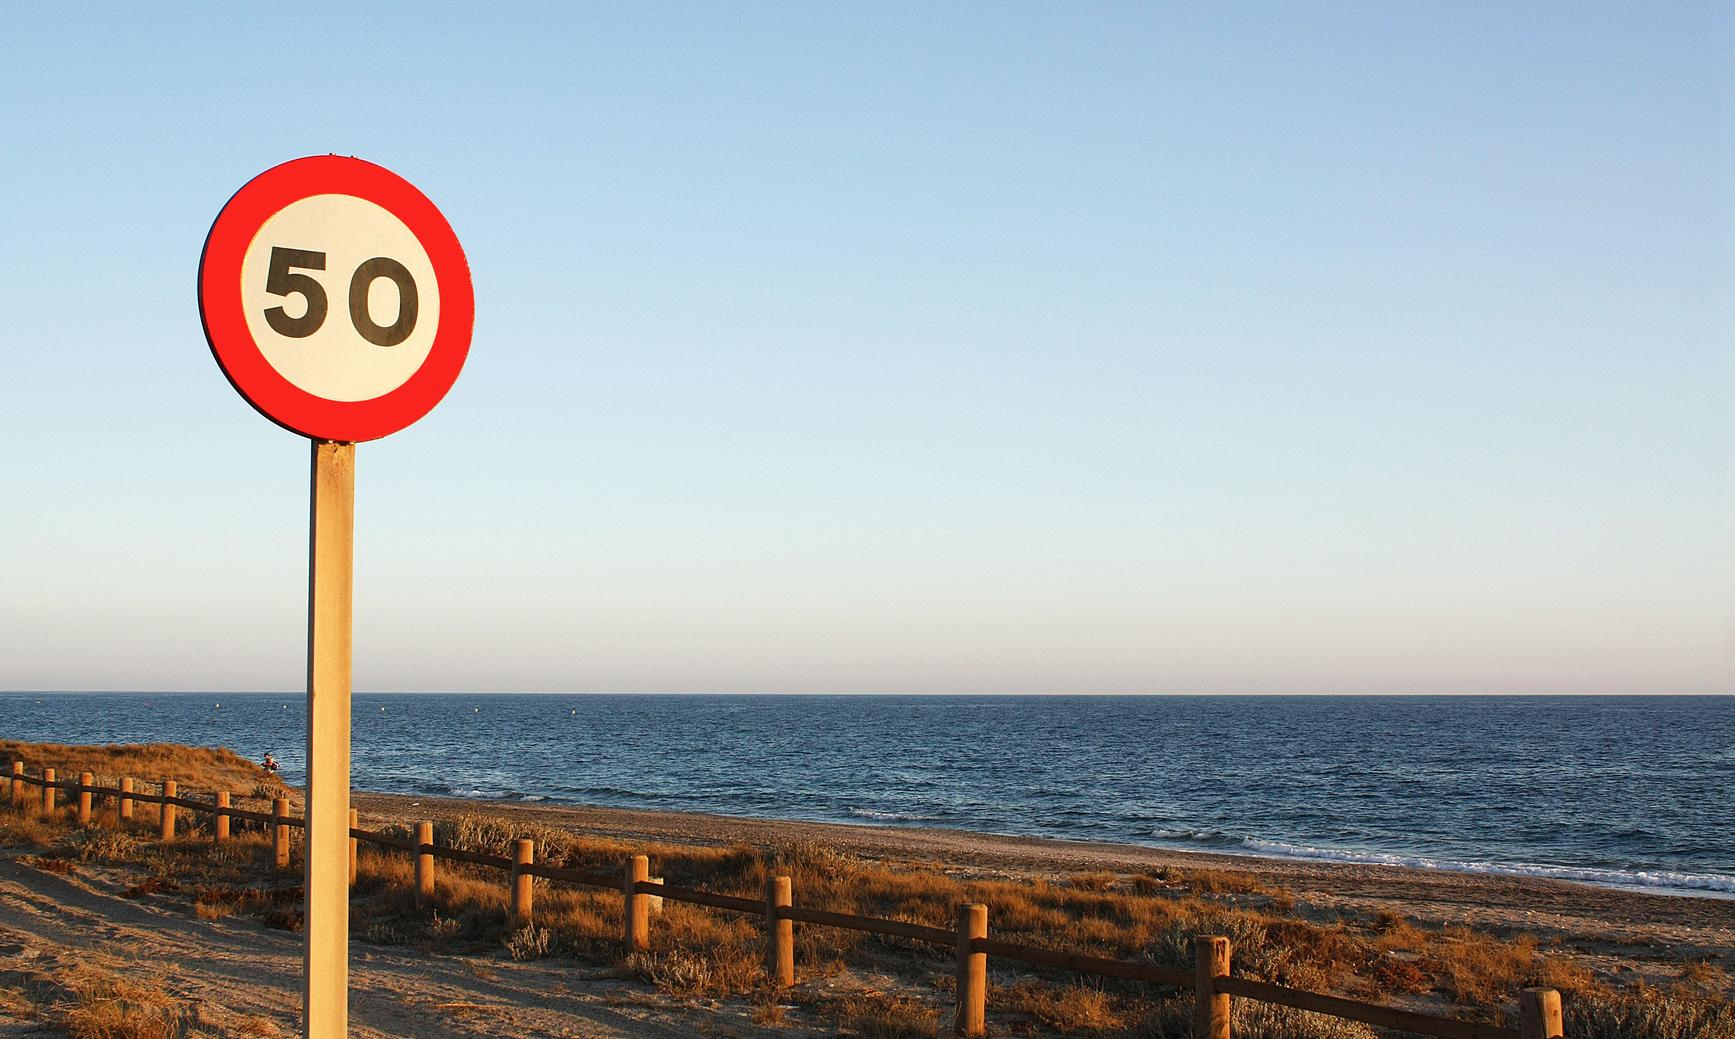
\includegraphics[width=0.35\textwidth]{./img/traffic_sign_s.jpg} &
		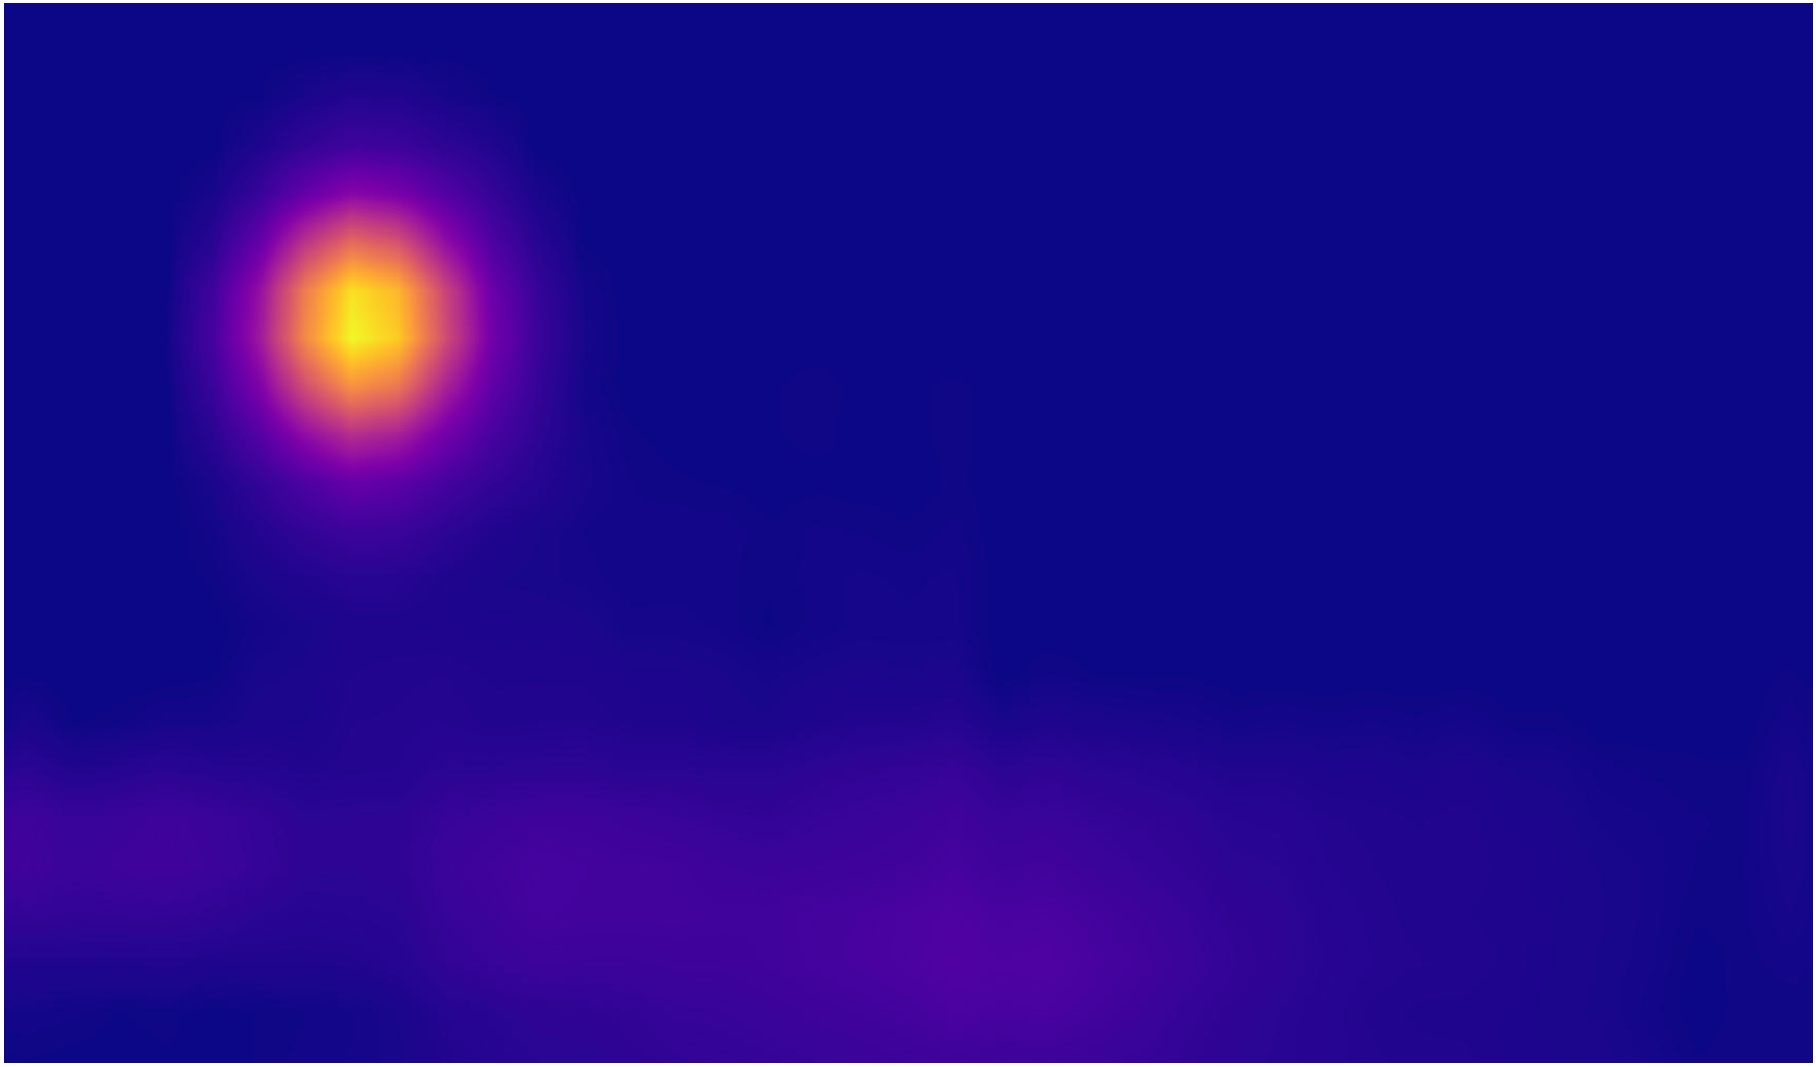
\includegraphics[width=0.35\textwidth]{./img/traffic_sign_m.jpg}\\
        (a) & (b)
		\end{tabular}
\end{center}
\caption{Example of visual saliency.
    b) is the salience map where brighter pixels represent regions more
    salient to humans on the original image a).}
\label{fig:example}
\end{figure}

Visually salient regions on images are usually represented by
\emph{saliency maps} (Figure~\ref{fig:example}). In these maps, images are generated such that
areas with high-valued pixels express high saliency on the original image,
whereas regions with low-valued pixels represent low saliency.
Datasets with such maps are obtained by collecting eye-fixation
data from humans while observing the scenes.

\subsection{Related work}
Early computational models of visual saliency were generally built based on
filtering of images for extraction of a pre-selected set of features
considered important for \emph{bottom-up} attention.
\emph{Vocus}~\cite{frintrop_2005} is a computational model that extracts
features shown to be naturally salient to humans such as color/luminance
contrast and orientation from different scales of the image.

A rapid change of paradigm occurred around 2015 when \emph{Deep Learning}
techniques showed to be very effective in the generation of saliency
maps.
Models such \emph{Salicon}~\cite{jiang_2015} demonstrated that the use of 
convolutional neural networks with weights initialized from
image classification networks, e.g. \emph{VGG-16}~\cite{zisserman_2014}
could lead to salience maps very similar to those generated from humans.
\emph{ML-Net}~\cite{cornia_2016} uses the output of different layers
of \emph{VGG-16}, combining them in many dimensions and various levels of
abstraction. \emph{DeepFix}~\cite{kruthiventi_2015} extends a pre-trained model with
new layers that account for global features and center bias, whereas \emph{Salnet}~\cite{pan_2016} explores two models that are
simple yet provide good results. These models are usually evaluated and ranked on
\emph{MIT saliency benchmark}~\cite{mit_sal_bm}, which uses a variety of
metrics to express how close generated saliency maps are to those created from
human data. As of today, at least nine out of the ten best models in the ranking use
Deep Learning.

\subsection{Motivation}
Current state of the art models are in general quite expensive computationally,
partly because most of them are based on very big pre-trained networks.
The convolutional layers of \emph{VGG-16} are composed of around 14.7
million parameters.
While pre-trained weights from classification tasks showed to be effective
for saliency prediction, it is reasonable to question whether
creating a proper network from scratch could yield a smaller amount of
parameters that are more efficient for the sole task of salience prediction.
Also, there are some ideas from previous work on psychology-based models that were not
used in current models but that are considered worthwhile to explore.

\subsection{Objectives}
This work aims at building a visual saliency model that is a) effective,
yielding results similar to other state of the art models,
and b) relatively simple and computationally efficient.
It is important that both criteria are matched because we aim at extending the
model in the future for video and real time applications such as
navigating robots.

\section{Proposed model}
Figure~\ref{fig:model} shows the overall architecture of the fully
convolutional neural network proposed in this work.
It extracts features from increasingly smaller dimensions of the
input image.

\begin{figure}[hbt]
    \centering
    \def\svgwidth{0.9\columnwidth}
    \input{./img/model.pdf_tex}
    \label{fig:model}
    \caption{Overview of the network.
        Filters sizes are in format width$\times$height\_stride.}
\end{figure}

The network is composed of four main blocks:

\textbf{The first} level extracts low level features from the input image, of
        dimensions $W\times H \times 3$ (width, height, depth), using
        a single layer with 48 convolution filters with ReLu activation
        followed by max-pooling that reduces image by a factor of two.
        It was found that further decreasing the number of filters in this
        layer considerably hurts performance, which makes sense because it is
        important to capture high spatial frequency and high contrast
        information in the context of visual saliency.
\textbf{The second} level extracts low-medium level features from the
        input of dimensions $W/2 \times H/2 \times 48$ using two layers
        with 64 and 96 convolution filters, respectively, followed by ReLU
        activation and max-pooling.
		\textbf{The third }level extracts medium-high level features from input with
        dimensions $W/4 \times H/4 \times 96$ using four convolution layers.
        The first two layers have 128 filters each whereas the last two have 144 filters
        each. Every convolution layer is followed by ReLu.
        Max-pooling is carried out at the end.
        A considerable depth in this level was found to be important for
        the network's performance.
\textbf{The fourth} and last level is composed of eight inception blocks
        that extract high level features from the input with
        dimensions $W/8 \times H/8 \times 144$.
        Great level of depth and Inception blocks were found to be very
        important at this level.
        A $1 \times 1$ convolution makes a linear combination of the output
        maps at the end of the 8 inception blocks, followed by ReLu, producing
        the final saliency map of dimensions $W/8 \times H/8 \times 1$.

\begin{figure}[!htb]
    \centering
    \def\svgwidth{0.57\linewidth}
    \input{./img/inception.pdf_tex}
    \caption{Inception block layout.}
   \label{fig:newinception}
\end{figure}

Figure \ref{fig:newinception} illustrates the inception
architecture~\cite{szegedy_2014}
used in each block where filters of size $5 \times 5$, $3 \times 3$
(both preceded by $1\times 1$ convolutions in order to reduce the number
of input filters), $1 \times 1$, and a max-pooling of size $3 \times 3$ are applied.
Each of these operations is executed in parallel from the same input
and the outputs are concatenated at the output.
Inception allows the network to use
information from different spatial dimensions as well as previous
layers (lower level saliency information) in the final map
computation, which is considered to be important for visual saliency.
The network has a total of $3717841$ parameters, a very low number
compared to other models. Table \ref{table:inception} details the filter configuration for the inception layers.

\begin{table}[H]
\centering
	\small
\label{table:inception}
\caption{Number of filters used in each inception block.}
\begin{tabular}{|c|c|c|c|c|c|c|}
	\hline
    Block & pool & conv 1$\times$1 & 3$\times$3 reduce &
    conv 3$\times$3 & 5$\times$5 reduce & conv 5$\times$5\\
    \hline
    1 & 96 & 128 & 96 & 192 & 58 & 96\\
    \hline
    2 & 64 & 128 & 80 & 160 & 24 & 48\\
    \hline
    3 & 64 & 128 & 80 & 160 & 24 & 48\\
    \hline
    4 & 64 & 128 & 96 & 192 & 28 & 56\\
    \hline
    5 & 64 & 128 & 96 & 192 & 28 & 56\\
    \hline
    6 & 64 & 128 & 112 & 224 & 32 & 64\\
    \hline
    7 & 64 & 128 & 112 & 224 & 32 & 64\\
    \hline
    8 & 112 & 160 & 128 & 256 & 40 & 80\\
    \hline
\end{tabular}
\end{table}

\subsection{Implementation}
The network was implemented using \emph{Theano} \texttt{0.9.0.dev}
along with \emph{Lasagne} \texttt{0.2.dev1}
on a machine with \emph{Ubuntu 16.04 LTS} and
kernel \emph{Linux} \texttt{4.8.0-54-generic}.
Training was conducted on a GPU \emph{NVIDIA GTX 1080} and the
code is available at \texttt{https://goo.gl/WzpyYJ}.

\subsection{Training}
During training, the input images were resized to dimensions $320\times240\times3$.
Moreover, each image is normalized channel-wise by the subtraction of the channel mean and
division by the standard deviation. Besides, two aspects are worth mentioning in this pre-training phase: the use of normalizations per image, rather than per dataset, and the conversion of the images colorspace to the LAB colorspace. The choice regarding normalization was made because visual saliency is highly connected to the context of the image, hence saliency depends on the local context.
As for the colorspace, \emph{Vocus}~\cite{frintrop_2005} cites that the LAB colorspace is more
closely related to human vision once it encompasses red-green, yellow-blue and
luminance maps. We conjecture that this colorspace facilitates extraction of
important luminance and color contrasts by the learned convolution filters.
Prior experiments conducted by our group showed better performance using image-wise
normalization and LAB instead of the commonly used RGB\@.

In order to evaluate the model, the \emph{Correlation Coefficient} between the ground-truth saliency map $G$ and
the predicted map $P$: $CC(P, G) = cov(P, G)/(\sigma(P)\sigma(G))$ was considered.
In fact, there is a variety of metrics for evaluating saliency
predictions~\cite{judd_2016}, but $CC$ is considered one of the most appropriate
because it symmetrically penalizes both false positives and false negatives. However, other typical metrics were also evaluated (as it can be seen in \ref{table:results}).

For training, two datasets were considered:
\emph{SALICON}~\cite{jiang_2015}, with 15000 images, and
\emph{Judd}~\cite{judd}, with 1003 images.
The network was trained using Stochastic Gradient Descent with Nesterov
Momentum of $0.9$. SALICON was first used with data augmentation by flipping images
horizontally and vertically and the target normalized by mean-std
(Last conv layer had ReLu removed in this step).
Mean-std normalization of targets was applied because it led to faster convergence.
Training iterated for 5 epochs with learning rate of $0.009$
and then for 3 epochs with learning rate of $0.001$. Then, we switched to using unit normalization on targets.
The network was trained for 1 epoch with learning rate of
$3\times10^{-5}$ and L2 regularization of $10^{-4}$. Finally, Judd dataset was used with data augmentation by flipping images horizontally and the target normalized by unit normalization.
Training iterated for 2 epochs with learning rate of
$5\times10^{-5}$ and L2 regularization of $3\times10^{-5}$. Batch sizes were 10 for SALICON and 2 for Judd. The complete training process took around two and a half hours.

\section{Results}
Prediction took an average time of 8 milliseconds. Figure~\ref{fig:preds} shows some maps generated by the proposed model.
They are generally considerably similar to the ground truth. For evaluation, we submitted the model to the \emph{MIT300 saliency benchmark} that has around 300 images and is commonly used to rank such models. Table~\ref{table:results} shows the resulting values for the most common metrics. 
The proposed model achieved results comparable to those of the state of the art while having, at least, one fourth of the number of parameters.

\section{Conclusion}
In this paper, we proposed a novel fully convolutional neural network for the
prediction of visual saliency on images. The proposed model architecture and data preprocessing were designed specifically
for the task of salience prediction. Our methods showed to be effective, yielding to a network with performance
on \emph{MIT300 benchmark} consistently among the ten best results on various
metrics while having around $3/4$  less parameters than other state of
the art models.

\begin{figure}[hbt]
\begin{center}
		\begin{tabular} {ccc}
        Stimulus & Ground-truth & Proposed Model\\
		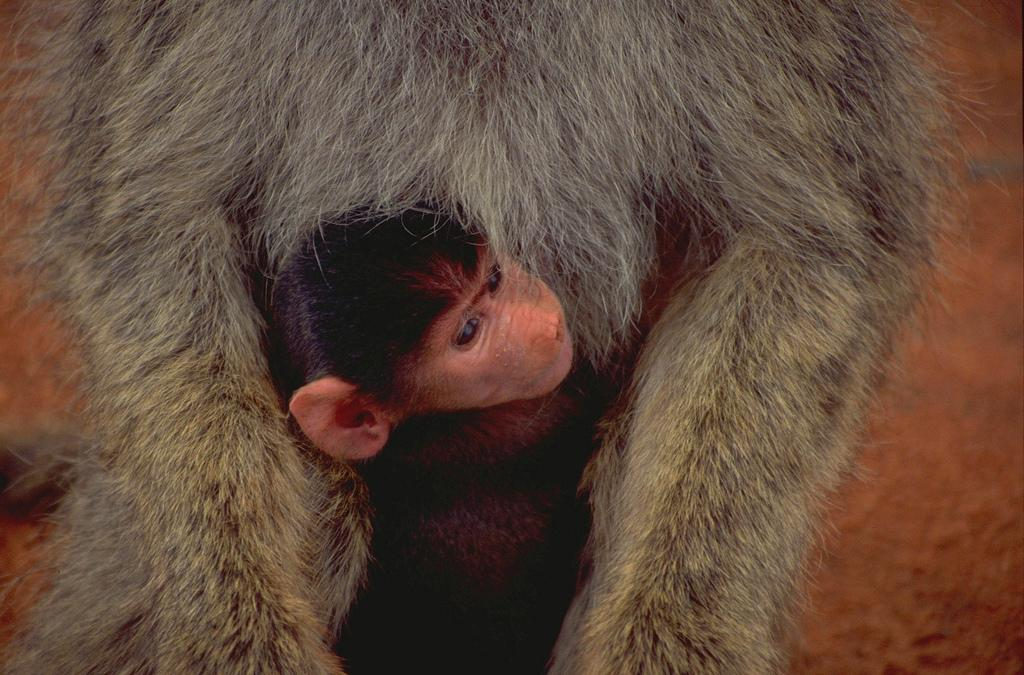
\includegraphics[width=0.19\textwidth]{./img/monkey_s.jpg} &
        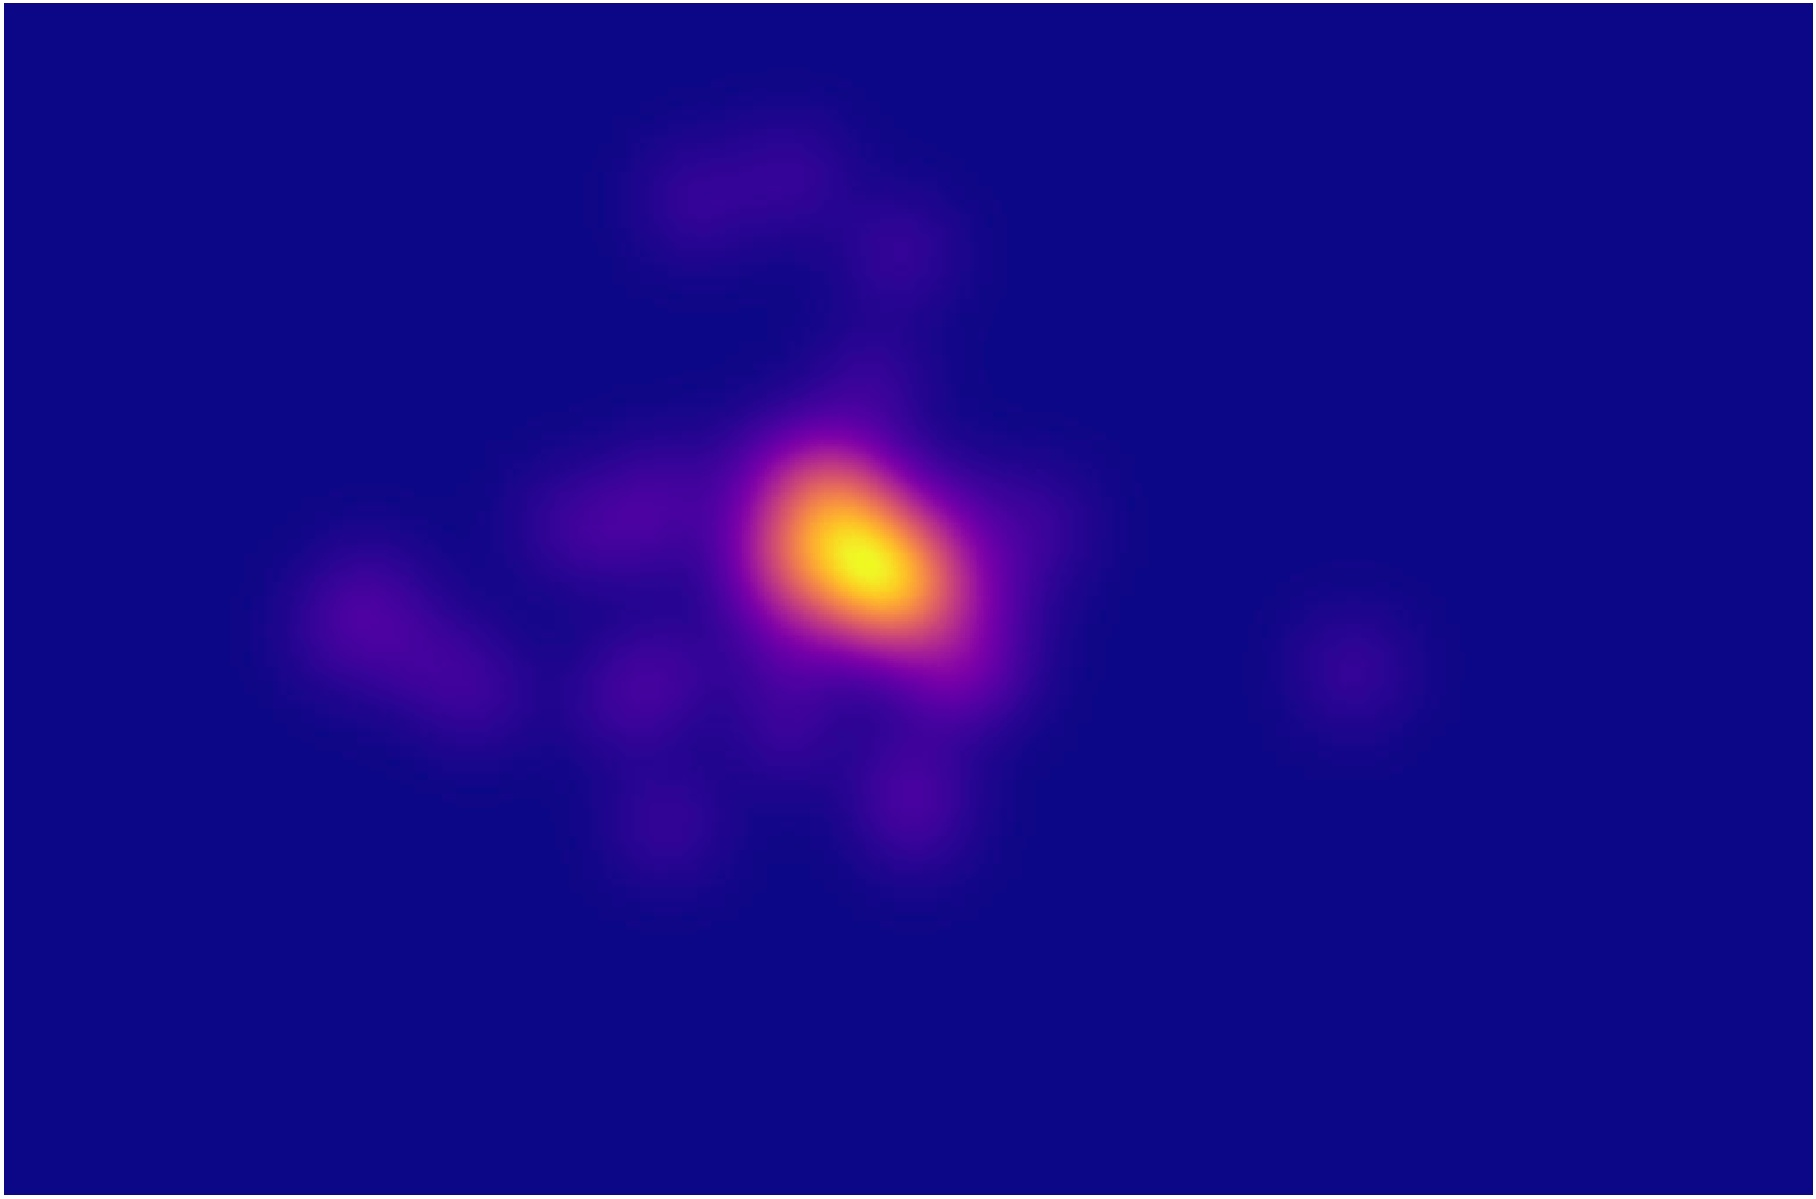
\includegraphics[width=0.19\textwidth]{./img/monkey_gt.jpg} &
		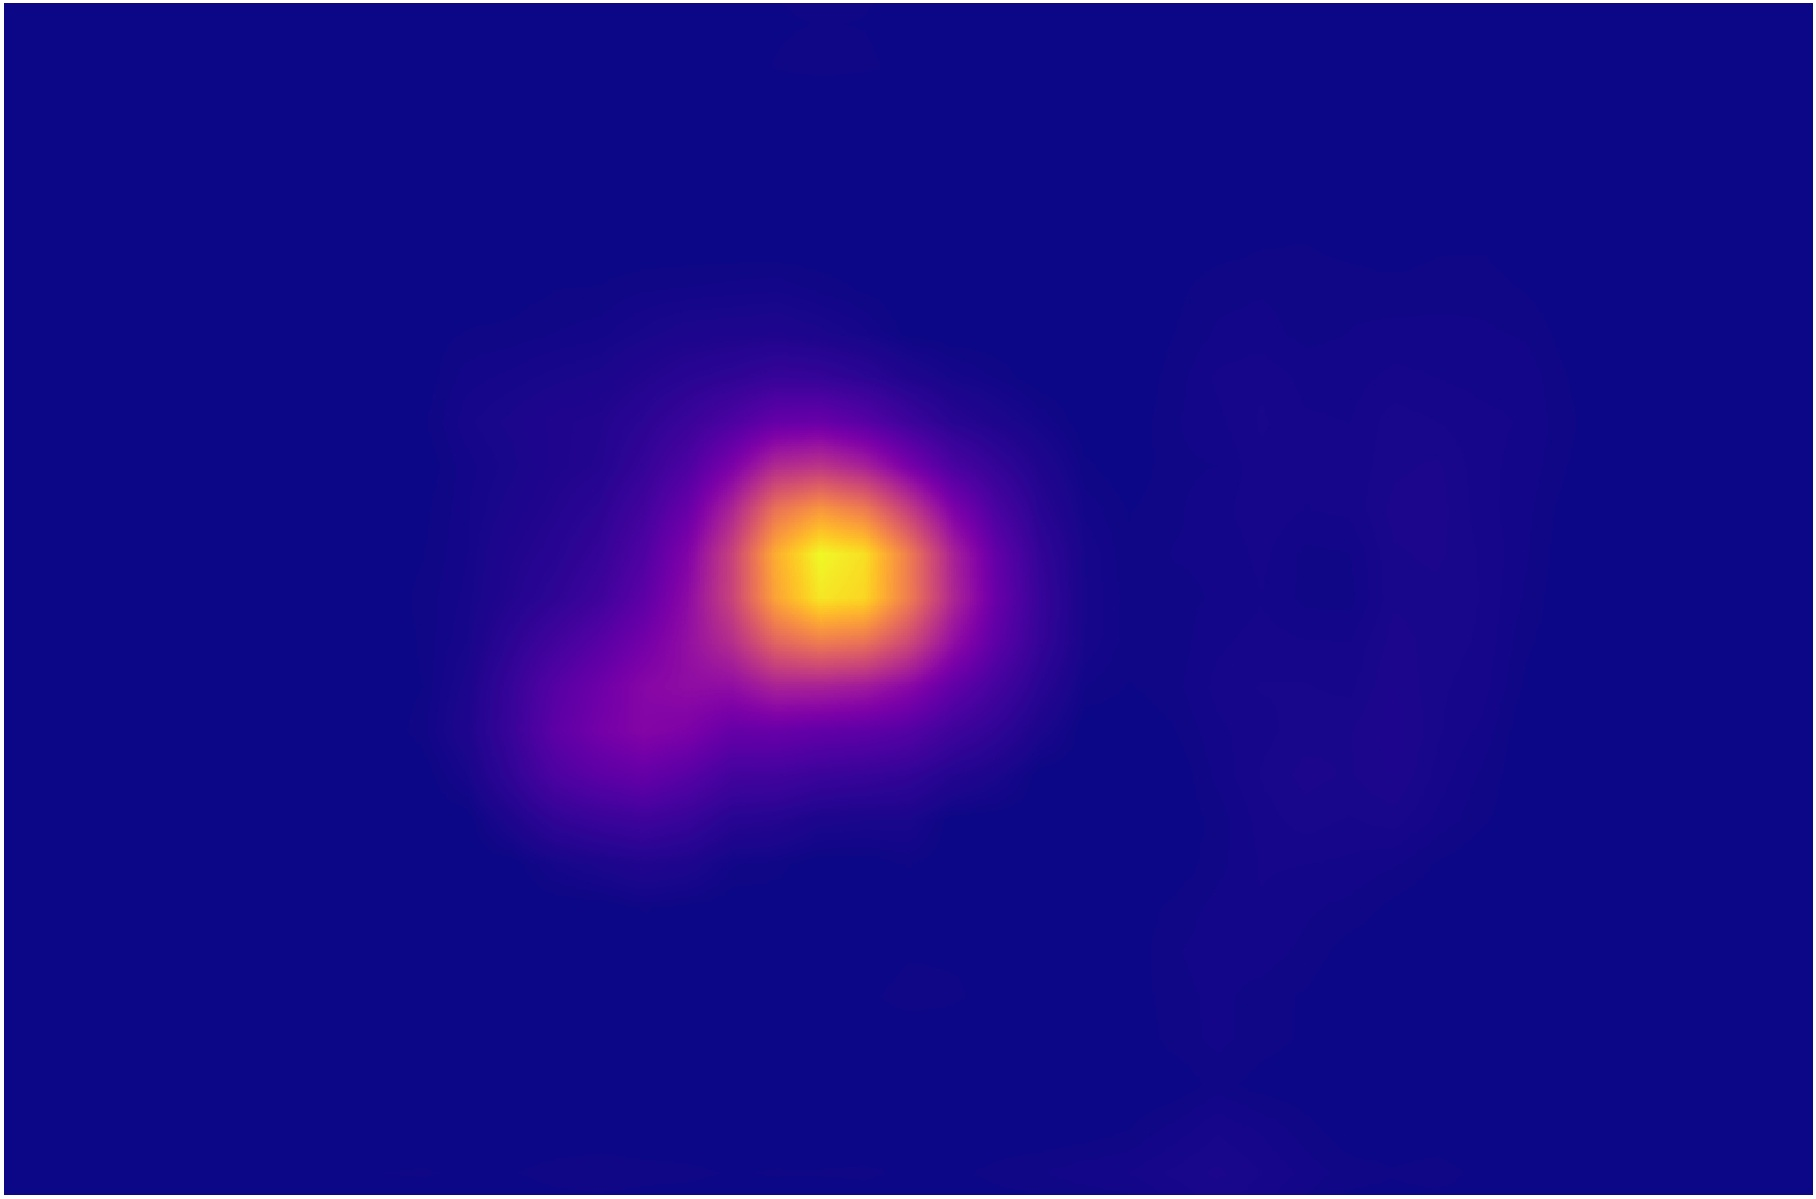
\includegraphics[width=0.19\textwidth]{./img/monkey_m.jpg}\\
		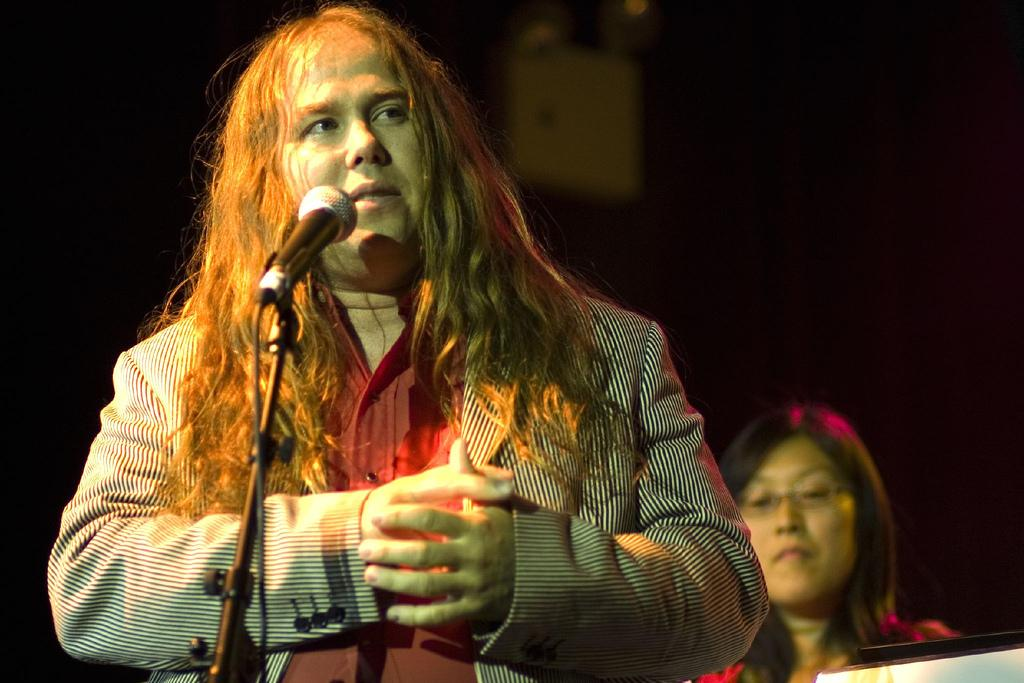
\includegraphics[width=0.19\textwidth]{./img/person_s.jpg} &
        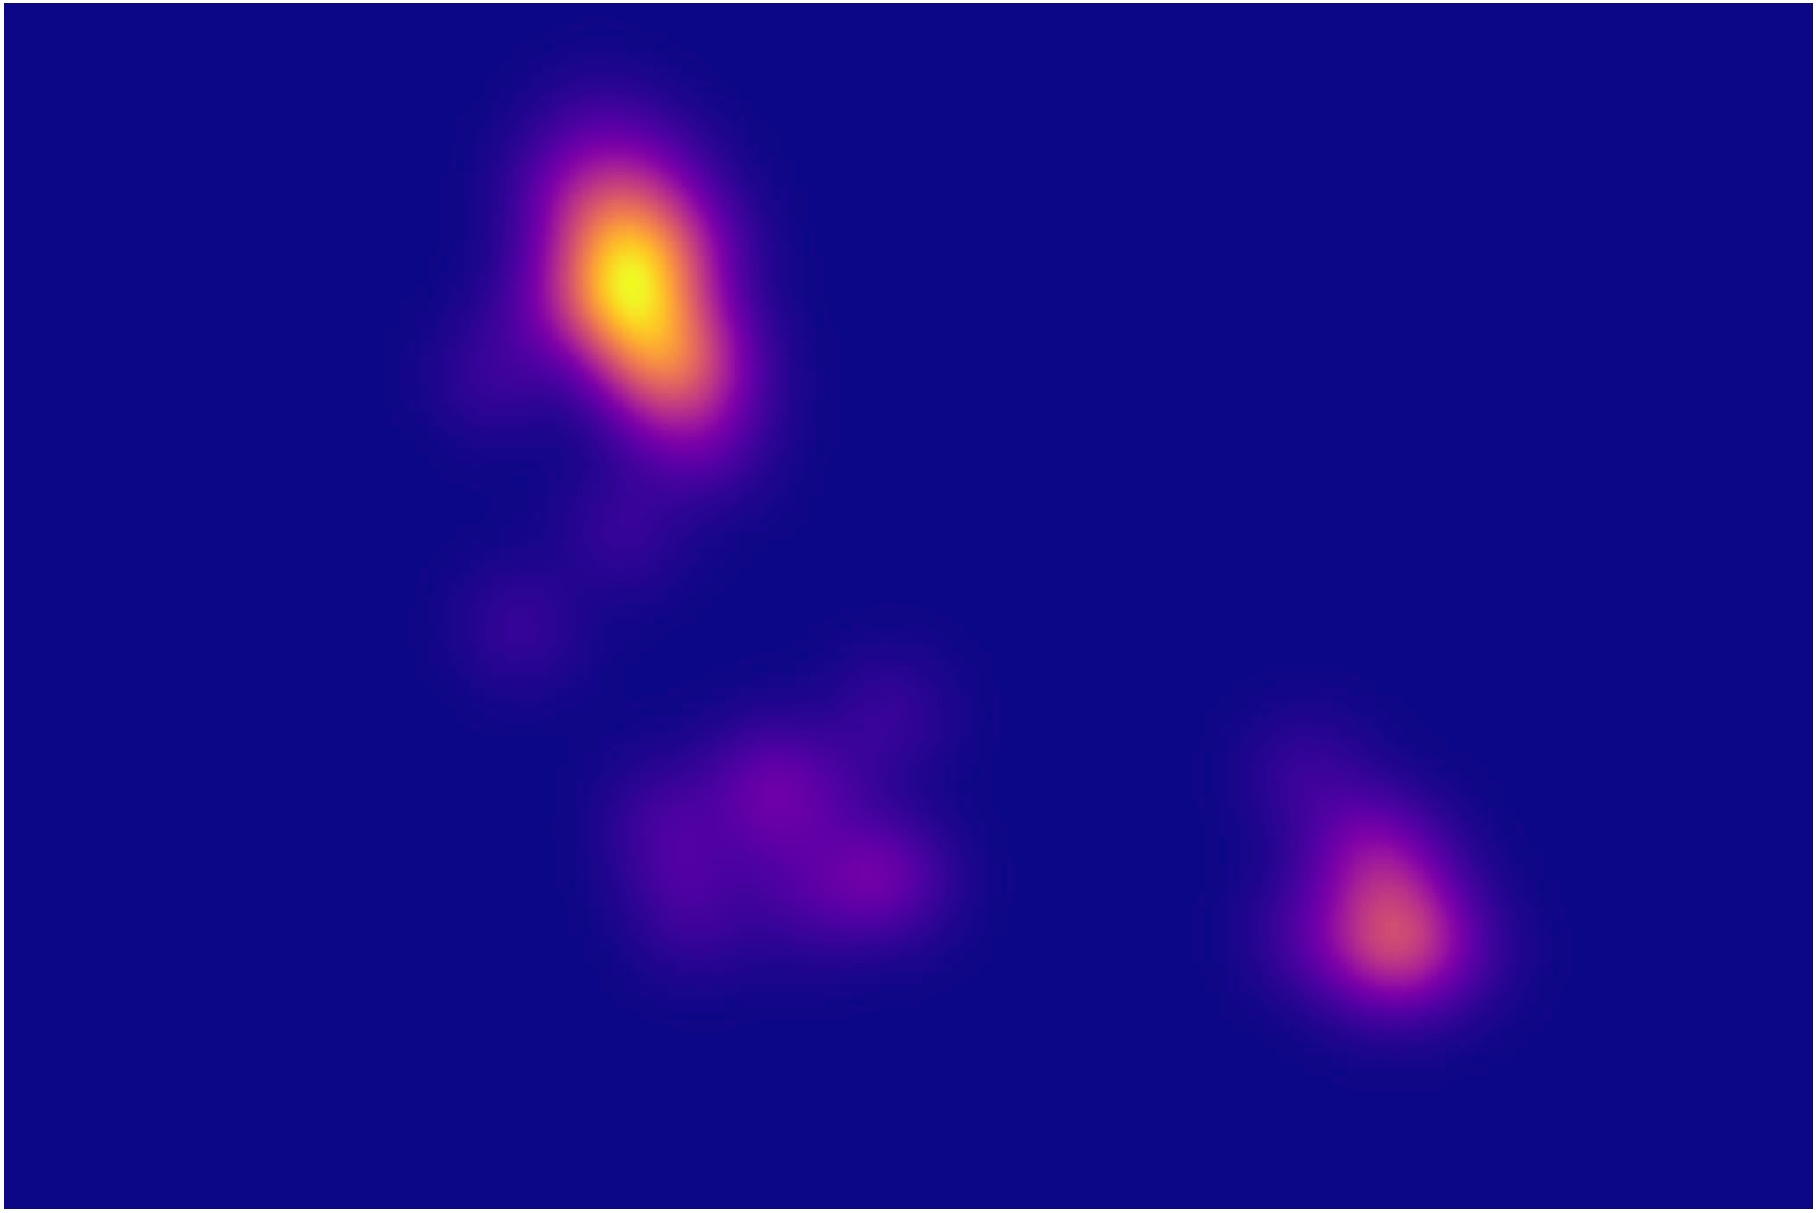
\includegraphics[width=0.19\textwidth]{./img/person_gt.jpg} &
		
\includegraphics[width=0.19\textwidth]{./img/person_m.jpg}\\
		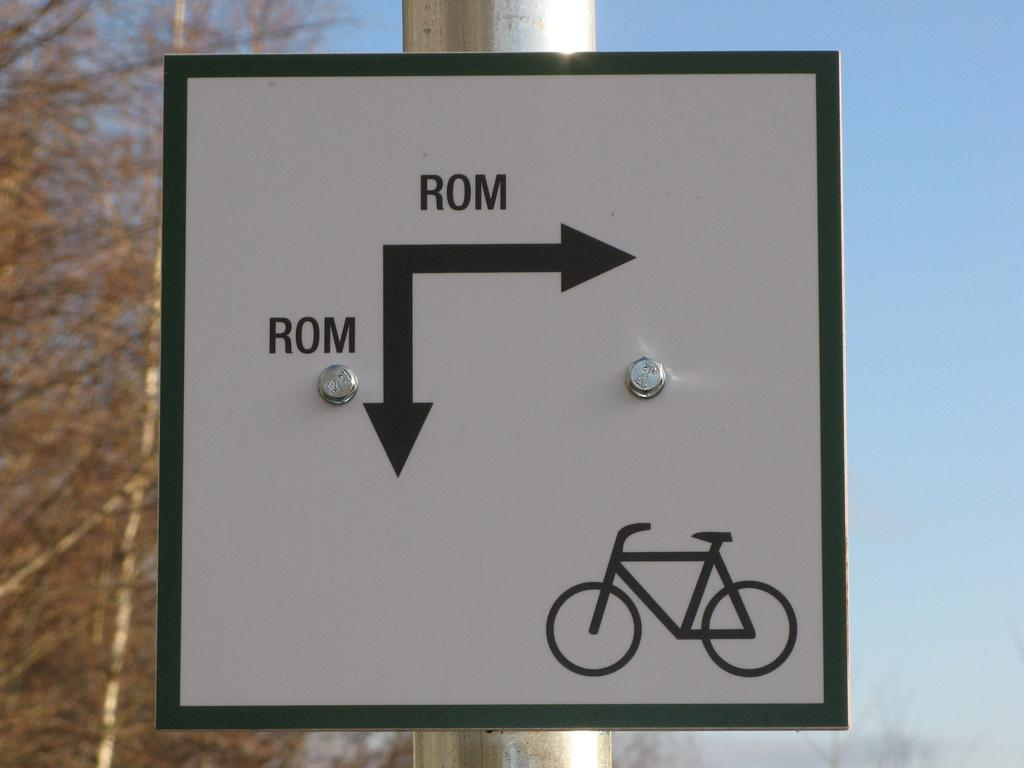
\includegraphics[width=0.19\textwidth]{./img/sign_s.jpg} &
        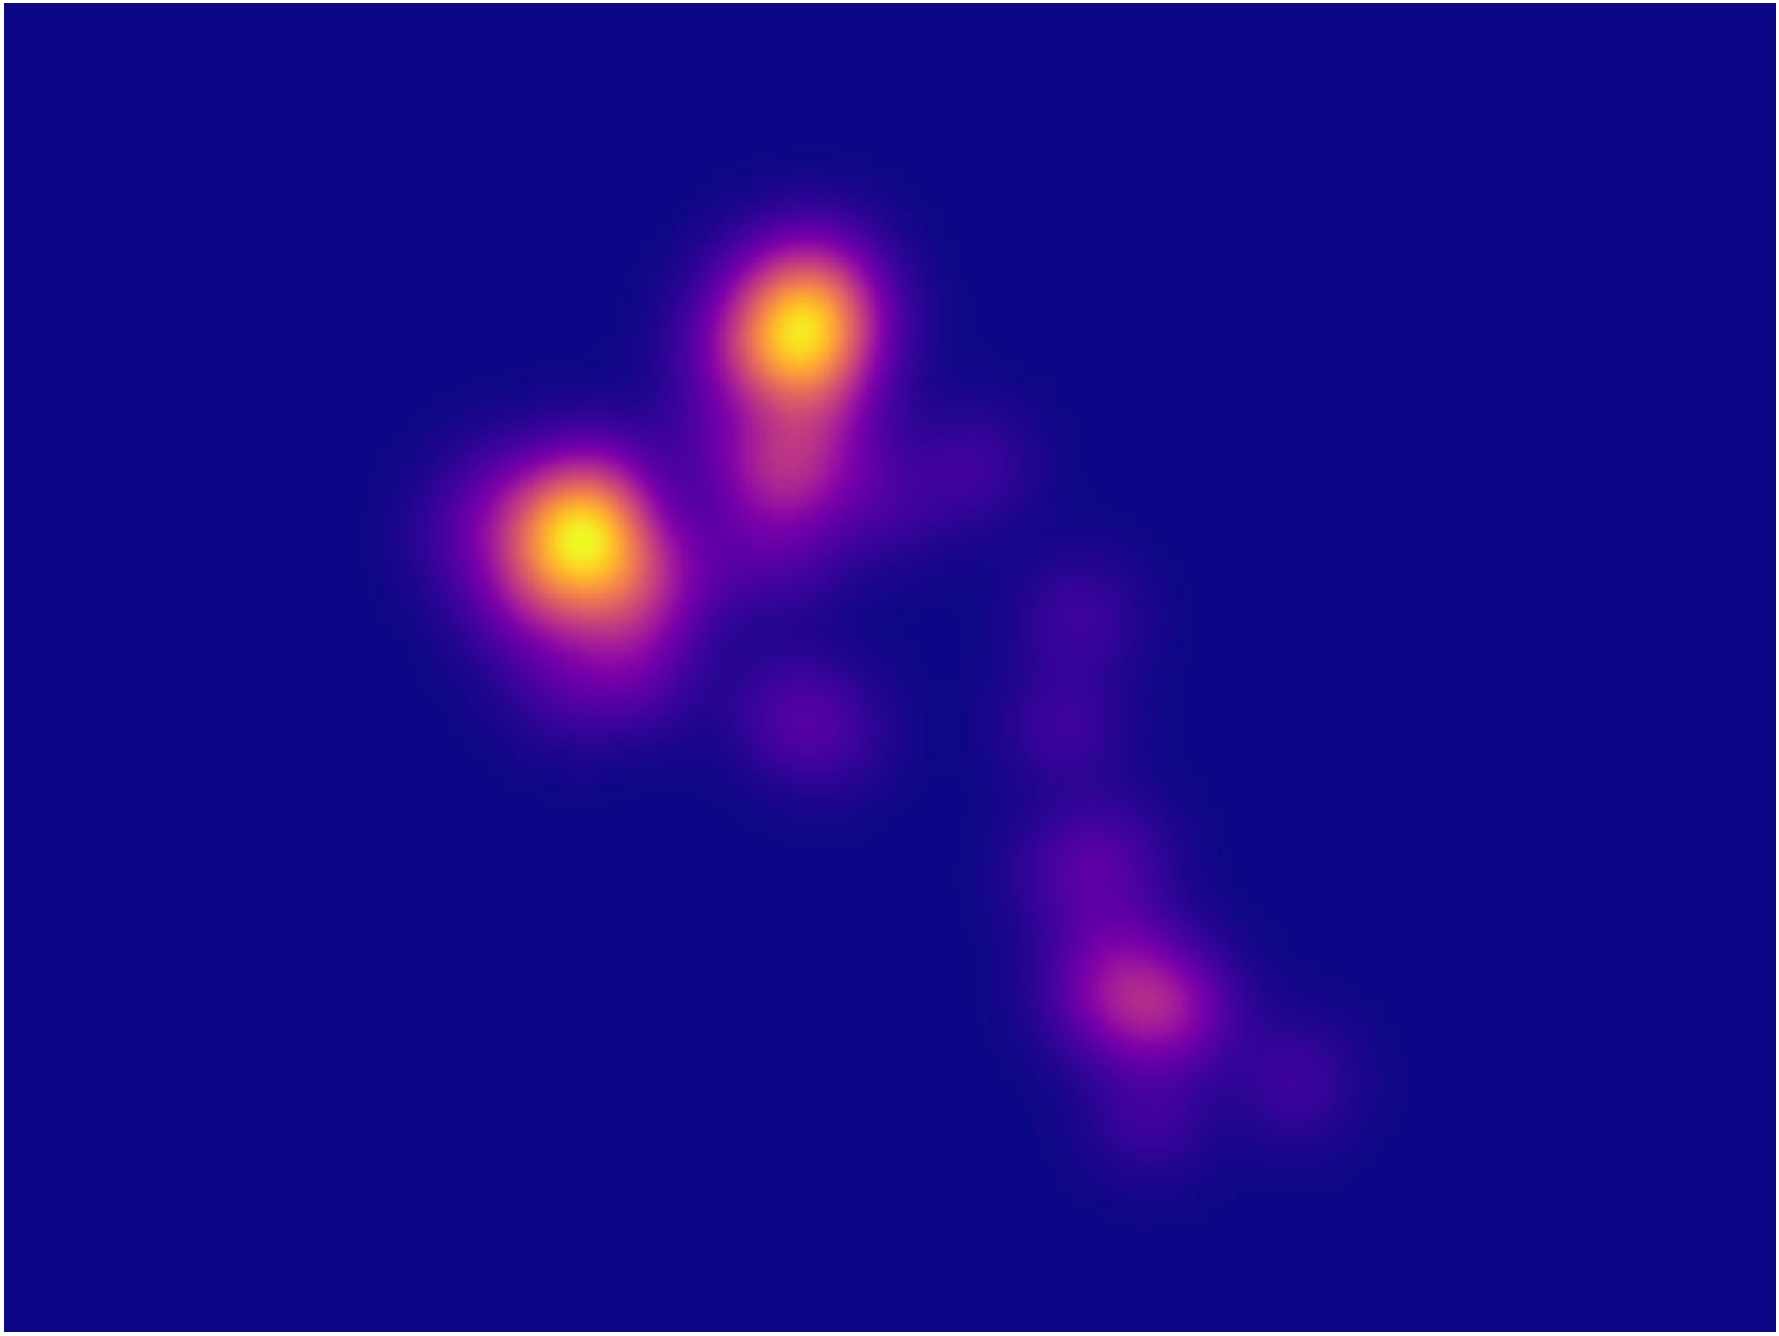
\includegraphics[width=0.19\textwidth]{./img/sign_gt.jpg} &
		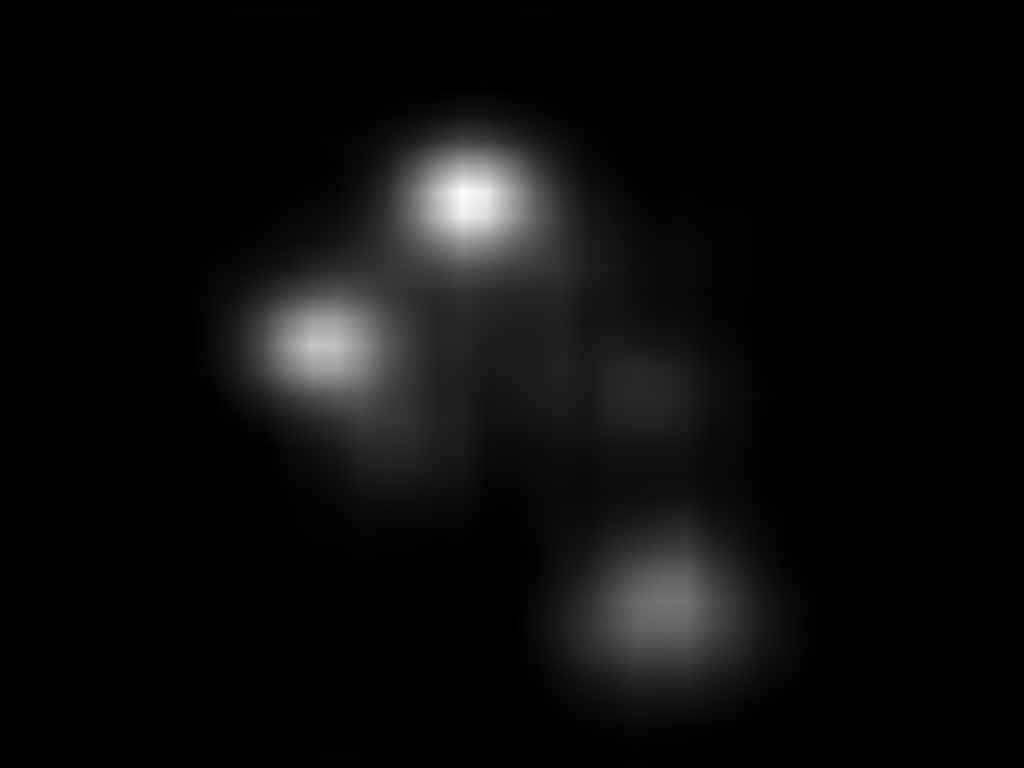
\includegraphics[width=0.19\textwidth]{./img/sign_m.jpg}\\
		\end{tabular}
\end{center}
\caption{Examples of predictions made by our model.}
\label{fig:preds}
\end{figure}


\begin{table}[!htb]
	\small
    \centering
    \label{table:results}
    \caption{State of the art models and metric scores on
    \emph{MIT300 benchmark}.}
    \begin{tabular}{|c|c|c|c|c|c|c|}
        \hline
        Model & Num. parameters & AUC-Judd $\uparrow$ & CC $\uparrow$
            & NSS $\uparrow$ & Sim $\uparrow$ & EMD $\downarrow$\\
        \hline
        Infinite humans & - & 0.92 & 1.0 & 3.29 & 1.0 & 0\\
        \hline
        \emph{DeepFix} & $\approx$16.7 million & 0.87 & 0.78
            & 2.26 & 0.67 & 2.04\\
        \hline
        \emph{Salicon} & $\approx$14.7 million & 0.87 & 0.74 & 2.12
            & 0.60 & 2.62\\
        \hline
        \textbf{Proposed Model} & \textbf{3.72 million} & \textbf{0.85} &
        \textbf{0.71} & \textbf{1.98} & \textbf{0.62} & \textbf{2.37}\\
        \hline
        \emph{ML-Net} & $\approx$15.4 million & 0.85 & 0.69 & 2.07 & 0.60
            & 2.53\\
        \hline
        \emph{SalNet} & 25.8 million & 0.83 & 0.57 & 1.51 & 0.52 & 3.31\\
        \hline
    \end{tabular}
\end{table}

% -- NAO MUDAR O ESTILO DAS REFERENCIAS BIBLIOGRAFICAS. O USO DO PADRAO DA SBC Eh OBRIGATORIO
\bibliographystyle{sbc}
\bibliography{bibliography}

\end{document}
